\documentclass[12pt, a4paper, headsepline]{article}
\usepackage[utf8x]{inputenc}
\usepackage[T1]{fontenc}
\usepackage[ngerman]{babel}
\usepackage{graphicx} 
\usepackage[automark]{scrpage2}
\usepackage{hyperref}
\usepackage{subfigure} 
\usepackage{ae} 
\usepackage{amsmath}
\usepackage{amsfonts}
\usepackage{amssymb}
\usepackage{floatflt}
\usepackage{pdfpages}
%\usepackage{fancyhd}
\usepackage{pdfpages}
\usepackage{listings}
\usepackage[style=super3colheader]{glossaries}
\usepackage{verbatim} %Mehrzeilige Kommentare durch \begin{comment} mglich  ??
\usepackage{blindtext} % Erzeugung von lngeren Textpassagen
\usepackage{xcolor}  

\definecolor{hellgrau}{rgb}{0.9,0.9,0.9}
\definecolor{darkgreen}{rgb}{0,0.5,0}
\definecolor{darkblue}{rgb}{0,0,2}

\lstset{inputencoding=utf8x, extendedchars=\true, numbers=left, numberstyle=\small, numbersep=5pt, basicstyle=\ttfamily\scriptsize, backgroundcolor=\color{hellgrau}, commentstyle=\color{darkgreen}, keywordstyle=\color{blue}, showspaces=false, showtabs=false, emph={String}, emphstyle=\color{blue}, emph={Boolean}, emphstyle=\color{blue}, showstringspaces=false}

\author{Andreas Paul}
\usepackage[bottom,hang]{footmisc}
\setlength{\footnotemargin}{0pt}
\addto{\captionsngerman}{\renewcommand*{\listfigurename}{}}
\makeatletter
\makeindex
\makeglossaries
\glsenablehyper 
\renewcommand{\entryname}{K\"urzel}
\renewcommand{\descriptionname}{Beschreibung}
%\renewcommand{\glspageheader}{S.}
\renewcommand*\l@section{\@dottedtocline{1}{1.5em} {2.3em}}
\renewcommand*\l@subsection{\@dottedtocline{2}{3.8 em}{3.2em}}
\renewcommand*\l@subsubsection{\@dottedtocline{3}{ 7.0em}{4.1em}}
\renewcommand*\l@paragraph{\@dottedtocline{4}{10em }{5em}}
\renewcommand*\l@subparagraph{\@dottedtocline{5}{1 2em}{6em}}
\renewcommand*\l@figure{\@dottedtocline{1}{1.5em}{ 2.3em}}
\newcommand{\pictext}[1]{\glqq\texttt{#1}\grqq }
% Abb. anstatt Abbildung verwenden %
\renewcommand{\figurename}{Abb.}
% Tab. anstatt Tabelle verwenden %
\renewcommand{\tablename}{Tab.} 
\renewcommand\subitem{\@idxitem \hspace*{30\p@}}
 % Tiefe der Nummerierung einstellen %
\setcounter{secnumdepth}{3} 
\setlength{\textheight}{660pt}
\addtolength{\voffset}{-40pt}
\makeatother 
\renewcommand{\refname}{Quellenverzeichnis} 
\linespread{1.50} %zeilenabstand 1.5}
\setlength{\headheight}{3.0\baselineskip}
\setlength{\fboxsep}{3mm}

\begin{document}
\setlength{\parindent}{0mm}

\includepdf{Titelblatt.pdf}
%\maketitle
\thispagestyle{empty}
\newpage 

\thispagestyle{empty}
\renewcommand{\contentsname}{Inhalt}
\tableofcontents
\thispagestyle{empty}

\pagestyle{scrheadings}
\ihead{
\includegraphics[width=0.06\textwidth]{bilder/fzk2.png}}
%\chead{\rightmark}
\chead{\leftmark}
\cfoot{Andreas Paul - Forschungszentrum Karlsruhe}

\newpage
 \cappclause{Andreas Paul}          % author name
        {Karlsruhe, den \today}    % location, date (for legal clause)
\newpage

\newglossaryentry{DMS}{name={DMS},description={Dokumenten-Management-System},text={DMS}}
\newglossaryentry{CMS}{name={CMS}, description={Content-Management-System},text={CMS}}
\newglossaryentry{ECM}{name={ECM}, description={Enterprise-Content-Management},text={ECM}}
\newglossaryentry{UCM}{name={UCM}, description={Universal-Content-Management},text={UCM}}
\newglossaryentry{AIIM}{name={AIIM}, description={Association for Information and Image Management - Die AIIM ist eine Gesellschaft von internationalen Herstellern und Anwendern von Informations- und Dokumenten-Mangement-Systemen.},text={AIIM}}
\newglossaryentry{SSH}{name={SSH}, description={Secure Shell - Durch eine Secure Shell kann man sich eine verschlüsselte Netzwerkverbindung zum entfernten Rechner aufbauen.},text={SSH}}
\newglossaryentry{LDAP}{name={LDAP}, description={Lightweight Directory Access Protocol},text={LDAP}}
\newglossaryentry{NSCA}{name={NSCA}, description={Nagios Service Check Acceptor},text={NSCA}}
\newglossaryentry{MIB}{name={MIB}, description={Management Information Base},text={MIB}}
\newglossaryentry{DNS}{name={DNS}, description={Domain Name System},text={DNS}}
\newglossaryentry{NRPE}{name={NRPE}, description={Nagios Remote Plugin Executor},text={NRPE}}
\newglossaryentry{OracleUCM}{name={OracleUCM}, description={Content-Management-System von Oracle},text={Oracle UCM}}
%%%%%
%
% glossary entries
%
%%%%% 

\pagenumbering{arabic}

\section{Einleitung}

Einleitung halt.
Kurz was ist Nagios, warum überhaupt überwachen?
Was soll überwacht werden -> Stellent/UCM kurz was ist das? Warum gerade das überwachen -> Aktive Benutzung durch User - kritisch 
\newpage
\section{Abstract}


Dokumenten-Management-Systeme bilden eine zentralen Dienstleistung im Karlsruhe Insitute of Technology.
Diese Systeme sind komplex aufgebaut und benötigen ausgefeilte Kontrollmaßnahmen / Überwachungsroutinen um einen stabilen Betrieb zu garantieren / ermöglichen.
Zum gegenwärtigen Zeitpunkt gibt es keine ausgereifte Überwachungssoftware, die diese Aufgabe zufriedenstellend erfüllt.

Diese Bachelorarbeit beschreibt die Entwicklung von neuen Werkzeugen für die Open Source-Überwachungssoftware Nagios um das Dokumenten-Management-System \gls{OracleUCM}\footnote{Oracle Universal-Content-Management} auf Fehlverhalten hin zu kontrollieren.
Diese sogenannten Plugins lassen sich in bestehende Nagios-basierende Systeme einbinden und erweitern deren Bandbreite an zu überwachenden Elementen.
Da Hauptaugenmerk lag dabei, auf der Simulation von Benutzerverhalten und der Erkennung der dabei auftretenden Fehler.
Die Verantwortlichen sollen durch die Benachrichtigung dieser Fehler sofort alarmiert werden und durch die unterschiedliche Tiefe der Überwachungstests die Problemquellen eingrenzen können.
%, welche möglichst zu Laufzeit erkannt und deren Fehl
%Meldungen können die Problemquellen vom Administrator gefunden und eventuell behoben werden,
%Diese Bachelorarbeit beschäftigt sich mit der Entwicklung eines Plugins für die Open Source-Überwachungsoftware Nagios intensiven Überwachung des Dokumenten-Management-Systems \gls{OracleUCM}\footnote{Oracle Universal-Content-Management} durch  um proaktiv auftretende Fehler zu entdecken.
%Dabei werden die Grundlagen von Dokumenten-Management-Systemen, Aufbau von \gls{OracleUCM} und Nagios beleuchtet und beschrieben.
%Dadurch kann eine geeignete Methode aus den unterschiedlichen Überwachungsmethoden von Nagios ausgewählt werden.
%Notwendige Kenntnisse über Service-orientierte Architektur (\gls{SOA}) und Web Services werden für die Umsetzung angeeignet.

Die Überwachung besteht aus den Ebenen: Statusabfragen, Funktionalitätstests, Auswertung von Logdateien und Benutzersimulation.
Auf dem Windows-Servers der \gls{OracleUCM}-Anwendung wird ein passender Nagios-Agent installiert, der aus einer vorherigen Übersicht ausgewählt wurde.
Die Konfiguration und der Einsatz von bereits erhältlichen Nagios-Plugins decken die ersten drei Ebenen ab.
Die automatisierte Benutzersimulation verwendet verschiedene Web Services der \gls{OracleUCM}-Anwendung.


%Ein Abstract ist eine prägnante Inhaltsangabe, ein Abriss ohne Interpretation und Wertung einer wissenschaftlichen Arbeit.

%Zusammenfassung von allem.

%Aufgabenstellung, Erwartendes Ergebnis
%\begin{itemize}
%\item Objektivität: soll sich jeder persönlichen Wertung enthalten
%\item Kürze: soll so kurz wie möglich sein
%\item Verständlichkeit: klare, nachvollziehbare Sprache und Struktur
%\item Vollständigkeit: alle wesentlichen Sachverhalte sollen explizit enthalten sein
%\item Genauigkeit: soll genau die Inhalte und die Meinung der Originalarbeit wiedergeben
%\end{itemize}
 \newpage
\section{Aufgabenstellung}
Oracle UCM werden im FZK eingesetzt, bisher nur rudimentäre Überwachung durch Nagios möglich.
Diese Arbeit soll die spezifischen Überwachungselemente erurieren und umsetzten. \newpage
\section{Grundlagen}
In diesem Kapitel werden die Grundlagen von Überwachungssystemen und Dokumenten-Management-Systemen erläutert.
Insbesondere wird auf Service-Orientierte Architektur (\gls{SOA}) und Web-Services für die spätere Umsetzung eingegangen.

%Wenn Du nicht "ich" schreiben willst kannst Du ja schreiben "wird diskutiert", "wird der Schwerpunkt gesetzt"...
%In diesem Kapitel werde ich die Grundlagen von Überwachungssystemen diskutieren und ...mit Schwerpunkt auf....Insbesondere werde ich näher eingehen auf...
\subsection{Überwachungssysteme}
\label{monitor}
Überwachungssysteme wurden für den Zweck entwickelt den Status von verschiedenen Objekten meist über das Netwerk zu überwachen und im Falle einer Statusänderung diese Information an die zugewiesenen Kontaktpersonen weiterleitet.

Bei diesen Objekten kann es sich um viele verschiedene Komponenten handeln.
Generell unterscheidet man zwischen der Überwachung ermöglichten zu Grunde liegenden Hardware den so genannten Hosts und den auf diesen Hardwarekomponenten aufsitzenden Diensten auch Services genannt.

Unter Hosts fallen nicht nur Server bzw. Computer, sondern auch Switches, Router oder auch dedizierte Überwachungshardware wie Sensoren für Temperatur, Luftfeuchtigkeit oder Rauchmelder.
Die Services dieser Hosts weichen je nach Art der Hosts stark voneinander ab.
Auf einem Server kann als Service ein Webserver im Betrieb sein, dessen Funktionalität sich simpel über einen Aufruf einer Webseite überprüfen lässt.
Bei einem Switch können beispielsweise als Service die Übertragungsrate, der Paketverlust oder der Portzustand überwacht werden.

Sehr wichtig ist bei einem Überwachungssystem die Gewichtung der erhaltenen Überwachungsinformationen.


%\begin{center}
%was ist wichtig was nicht, Gewichtung, Klassifizierung, Organisationsstrategie
%Host,Services erklären
%\end{center}
\newpage
Vor der Einführung eines Überwachungssystems muss sich mit den folgenden Punkten auseinandergesetzt werden.

\subsubsection{Ressourcenbelastung}
Die Einführung einer Überwachungssoftware bringt bei größeren Serverlandschaften eine nicht zu verachtende Netzwerk- und Prozessorbelastung mit sich.
Dabei unterscheidet Josephsen die anfallende Belastung in zwei unterschiedliche Arten der Überwachung\footnote{Quelle: \cite{Jose07} S. 4}:

\paragraph{Zentralisierte Überwachung}
Die Durchführung der Überprüfungen findet durch einen zentralen Überwachungsserver statt, der die Informationen über die einzelnen Hosts und Services über das Netzwerk abfragt.
Diese Methode ist in der Regel vorzuziehen, da hierbei die zu überwachenden Geräte weniger belastet werden und die Konfiguration der einzelnen Kontrollschritte zentral möglich ist.

\begin{figure}[ht]
	\centering
	   \fbox{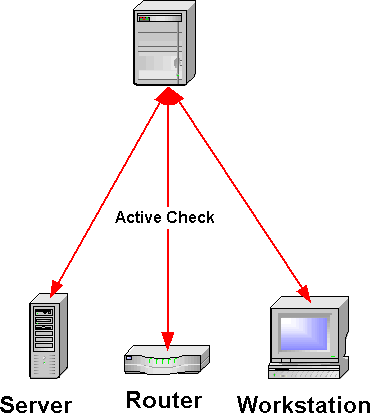
\includegraphics[width=0.5\textwidth]{bilder/dist_mon12.png}}
	   %\fbox{Quelle: \cite{Jose07} S. 5}
		\caption[Zentralistische Bearbeitung]{Zentralistische Bearbeitung}
		\label{distmon2}
\end{figure}
%\footnotetext{Quelle: \url{http://www.nagios-wiki.de/\_media/nagios/howtos/dist\_mon.png}}


\paragraph{Dezentralisierte Überwachung}
Bei einer sehr hohen Anzahl von zu überwachenden Objekten ist eine zentralisierte Ausführung nicht mehr von einem einzelnen Server tragbar.
In diesem Fall ist das Überwachungssystem darauf angewiesen, dass die einzelnen Hosts die kontrollierenden Überprüfungen selbständig durchführen und deren Ergebnisse an den Überwachungsserver weiterzuleiten.

%Kascadierende Überwachungssysteme kannst Du noch erwähnen

%Uberwachungsredundanzen vermeiden: Dein Beispiel mit dem Port führt in beiden Fällen dazu, dass der Test 1 überflüssig ist. Wenn die Webseite über 2 Ports abgefragt wird, z.B. 8000 Intranet, 8080 Internet, so wäre der Test 1 sinnvoll
\begin{figure}[ht]
	\centering
	   \fbox{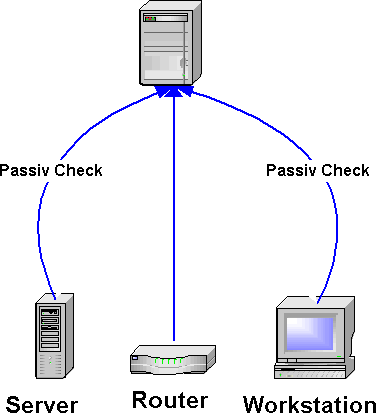
\includegraphics[width=0.45\textwidth]{bilder/dist_monp.png}}
	   %\fbox{Quelle: \cite{Jose07} S. 5}
		\caption{Ausgelagerte Bearbeitung}
		\label{distmonp}
\end{figure}

Um nicht komplett vom Überwachungsserver abhängig zu sein, kann ein zweiter Überwachungsserver bzw. weitere Server hinzugefügt werden.
Diese können bei einem Ausfall des Hauptüberwachungsservers die Verantwortlichen informieren oder die zu überwachenden Objekte zur Lastenteilung untereinander aufteilen.


%Nagios bietet zusätzlich noch eine weitere, dritte Möglichkeit durch das \textit{Distributed Monitoring} (Verteilte Überwachung) an, siehe Kapitel \ref{dismoni}.

\subsubsection{Netzwerkstruktur und Abhängigkeiten}
Die Überwachung von Hosts und Services über das Netzwerk erzeugt normalerweise immer zusätzlichen \gls{IP}-Traffic.
Das bedeutet, dass jede Überquerung weiterer Netzwerkknoten, die zwischen dem Überwachungsserver und den zu überwachenden Geräten liegen, eine weitere Belastung für das Netzwerk bedeutet, sowie eine Abhängigkeit zwischen Host und Server einführt.

\begin{figure}[ht]
	\centering
	   \fbox{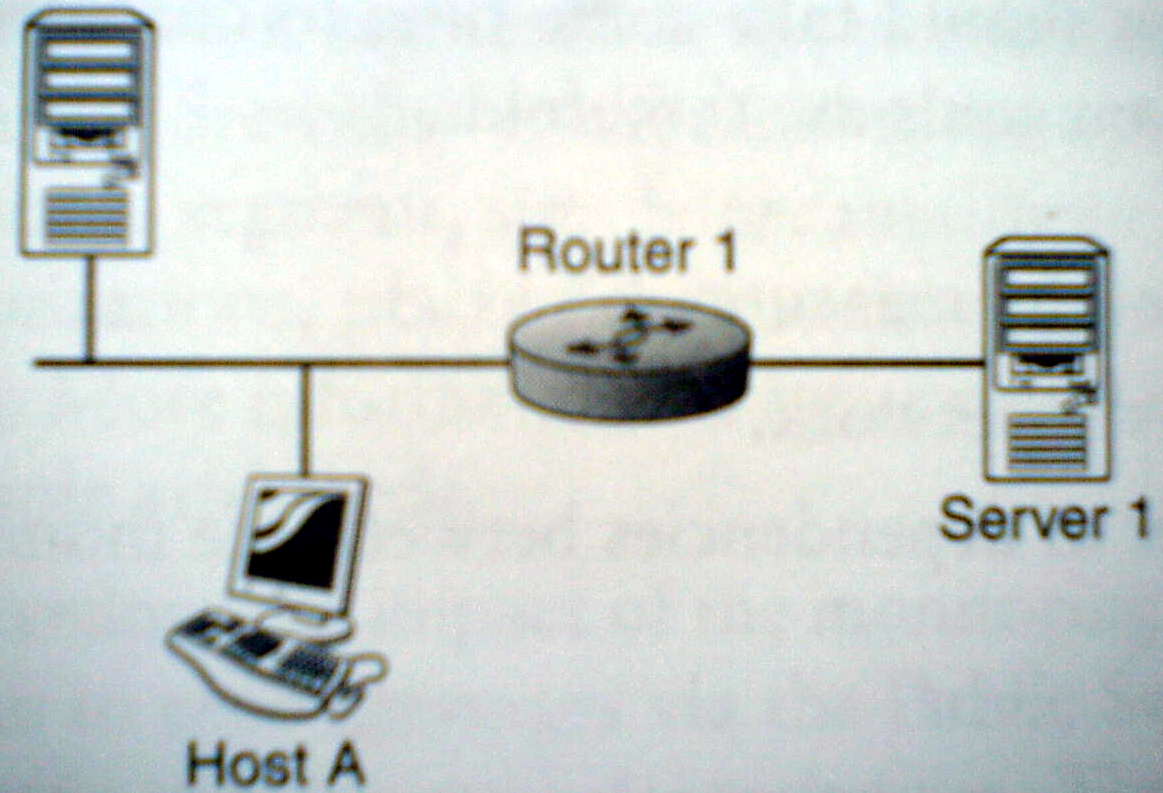
\includegraphics[width=0.5\textwidth]{bilder/dependent.png}}
	   %\fbox{Quelle: \cite{Jose07} S. 5}
		\caption[Zusätzliche Netzwerkabhängigkeit und Netzwerkbelastung]{Zusätzliche Netzwerkabhängigkeit und Netzwerkbelastung\protect\footnote}
		\label{depend}
\end{figure}
\footnotetext{Quelle: \cite{Jose07} S. 5}
\newpage
In der Abbildung \ref{depend} erzeugt der Router 1 die zuvor beschriebene zusätzliche Netzwerkabhängigkeit und Netzwerkbelastung, da der Server 1 bei einem Ausfall des Routers nicht mehr durch den Überwachungsserver erreichbar ist und jede Überprüfung, die vom Überwachungsserver gesendet wird den Router mit dem Routing der Pakete belastet.

Deshalb gilt es laut \cite{Jose07} S. 5 folgende zwei Punkte beim Erstellen eines Überwachungssystems zu beachten:

\paragraph{Überwachungsredundanzen vermeiden}
Redundante Überwachung entsteht dadurch, dass der gleiche Service durch zwei Arten mit unterschiedlichen Tiefen / Tiefgang geprüft wird.
Ein einfaches Beispiel ist die Überwachung eines Webservers auf dem Standardport 80.
Eine Überwachungsmethode ist es diesen Port abzufragen und die entsprechende Rückantwort des Servers auszuwerten.
Soll die auf dem Webserver laufende Webseite überwacht werden, kann die jeweilige Webseite über die Adresse nach einem bestimmten Inhalt untersucht werden.

In beiden Fällen wird getestet, ob der Webserver über das Netzwerk ansprechbar ist, jedoch sagt der zweite Test zusätzlich noch aus, dass die Webseite korrekt angezeigt wird, somit wäre der erste Test überflüssig.
Jedoch muss zuvor abgewogen werden, ob eine redundante Überwachung nicht sogar hilfreich bei der Ermittlung der Fehlerursache ist.
Wenn im oberen Beispiel der Inhalt der überwachten Webseite verändert wird, ist dies nur aus dem zweiten Test ersichtlich.
%, dass der Webserver einwandfrei funktioniert.

\paragraph{Minimale Netzwerkbelastung}
Um bereits stark belastete Netzwerkpunkte zu entlasten, bietet es sich an die Frequenz mit der die Test über das Netzwerk gesendet werden zu verringern.
Die Aufstellung des Überwachungsservers ist dadurch gerade bei größeren Serverlandschaften sehr wichtig, da durch eine effiziente Platzierung womögliche Flaschenhälse / Engstellen in Form von veralteten Switches oder ähnlichem vermieden werden können.

\subsubsection{Sicherheitsaspekte}
Um erweiterte Statusinformationen über einen Prozess oder über die Arbeitsspeicherauslastung auszulesen ist (meistens) zusätzliche Software auf den Hosts nötig.
Diese Software benötigt einen zusätzlichen geöffneten Port auf dem zu überwachendem Rechner, die einen neuen Angriffspunkt für Angreifer darstellen kann.
Außerdem erhält der Überwachungsserver Ausführungsrechte auf dem Client, so dass eine weitere potentielle Sicherheitslücke in einem (vermeintlich) zuvor sicherem System entsteht.
Jeder, der die Kontrolle über den Überwachungsserver besitzt oder sich als solcher ausgibt, kontrolliert somit gleichzeitig alle anderen überwachten Hosts.

Um dies zu verhindern gibt es verschiedene Ansätze.
Als ersten Ansatz sollte der Port durch den der Überwachungsserver mit dem Host kommuniziert vom Standardwert abweichen, damit nicht sofort erkennbar ist, dass sich eine (womöglich) angreifbare Überwachungssoftware auf dem Rechner befindet.\label{changeport}
Damit die über diesen Port versendeten Informationen nicht für Dritte zugänglich sind, bietet es sich an die auszutauschende Informationen mit einem Algorithmus zu verschlüsseln.
Durch den Einsatz eines Verschlüsselungsalgorithmus werden die Informationen nicht mehr im Klartext ausgetauscht, sondern
Da die Möglichkeit einer Verschlüsselung der Datenübertragung nicht von jeder Überwachungssoftware angeboten wird, gilt diese Option als Auswahlkriterium in der späteren Umsetzung bzw. im produktivem Betrieb. (Verweis auf Windows Agenten Übersicht?)

Des weiteren sollte die Erlaubnis der Abfrage der Überwachungsinformationen anhand der \gls{IP}-Adresse eingeschränkt werden, so dass der Client nur Anfragen des Überwachungsservers akzeptiert.
Durch diese Einschränkung kann vermieden werden, dass sensible Informationen aus den Antworten an unberechtigte Dritte übermittelt werden oder ein Denial of Service-Angriff (\gls{DoS}) durch eine übermäßig hohe Anzahl an Anfragen an den Client gesendet wird, um eine Überlastung des Servers zu erreichen und diesen somit arbeitsunfähig zu machen.

%\begin{itemize}
%\item Verschlüsselung der Informationen, die zwischen dem Server und dem Host hin- und hergesendet werden, damit man nicht die Inforamtionen im Klartext einfach auslesen kann.
%\item Firewall regeln, dazu Bild aus dem Jose07 Buch S9
%\end{itemize}
%\subsubsection{Port- versus Anwendungsüberwachung}
%\begin{itemize}
%\item E2E
%\end{itemize}






























\subsection{Dokumenten-Management-Systeme}

Um ein Dokumenten-Management-System (\gls{DMS})  zu erläutern muss sich zuerst mit dem Begriff des \textbf{"`Dokuments"'} auseinander gesetzt werden.
In \cite{DMS08} S. 2 wird ein Dokument durch folgende Punkte definiert:

\begin{itemize}
\item Ein Dokument fasst inhaltlich zusammengehörende Informationen strukturiert zusammen, die nicht ohne erheblichen Bedeutungsverlust weiter unterteilt werden können. 
\item Die Gesamtheit der Information ist für einen gewissen Zeitraum zu erhalten.
%item Dokumente dienen oft dem Nachweis von Tatsachen.
\item Ein Dokument ist als Einheit ablegbar (speicherbar) und/oder versendbar und/oder wahrnehmbar (sehen, hören, fühlen).
\item Das Dokument ist eigentlich der Träger, der die Informationen speichert, egal ob das Dokument ein Stück Paper, eine Datei auf einem Rechner, ein Videoband oder eine Tontafel etc. ist. Dies bedeutet auch, dass es keine Bindung an Papier oder ein geschriebenes Wort gibt.
\end{itemize}

Des weiteren gibt es eine Differenzierung in zwei Definitionen:

\begin{quote}"`Als \textbf{Dokument im konventionellen Sinne} werden Dokumente bezeichnet, die als körperliches Dokumente (z. B. Papier) vorliegen, ursprünglich als körperliches Dokument vorlagen oder für die Publizierung auf einem körperlichen Medium vorgesehen sind.

Die Begrifflichkeit des \textbf{Dokuments im weiteren Sinne} erweitert den Begriff des Dokuments um semantisch zusammengehörende Informationsbestände, die für die Publikation in nicht-körperlichen Medien, z.B. Webseiten, Radio, Fernsehen o. ä. vorgesehen sind. Derartige Dokumente werden oft dynamisch gestaltet und zusammengestellt."' \begin{flushright}\cite{DMS08} S. 2\end{flushright}\end{quote}

Dabei müssen auch Daten und Dokumente voneinander abgegrenzt werden.
In \cite{DMS08} S. 33 werden Daten im Allgemeinen als eher stark strukturierte Informationen gesehen, wobei Dokumente zumeist aus unstrukturierte bis zu schwach strukturierte Informationen bestehen.
Eine eindeutige Klassifizierung eines vorhandenen Dokumentes ist jedoch nicht immer möglich, da sich oft Mischungen beider Klassen finden lassen.
Ohne die dazugehörigen Metadaten besteht ein Bild aus unstrukturierten Informationen, daher auch \gls{NCI}-Dokument für None-Coded Information genannt.

Die Einordnung, wann ein Dokument strukturierte oder unstrukturierte Informationen enthält, lässt an folgenden Beispielen verdeutlichen.
Bei einem Bild oder Foto lassen sich die enthaltenen Informationen ohne zusätzliche Metadaten nicht eindeutig durch Computer bestimmen.
%Beispielsweise, ob sich eine Person auf dem Bild befindet oder wann und wo das Foto erstellt wurde.
Daher ist ein Bild, solange keine Metadaten darüber bekannt sind, ein eindeutiges Beispiel für \gls{NCI}-Dokumente mit unstrukturierten Informationen.
Im Gegensatz dazu lassen sich die Werte einer Tabelle oder eines Datensatzes durch die Spaltennamen eindeutig bestimmen und durch den Computer auslesen.
Solche Daten mit strukturierten Informationen werden daher auch als Dokumententyp mit Coded Information (\gls{CI}) bezeichnet.

Der Anteil von strukturierten Informationen in einem Dokument nimmt von Bildern über Text zu Tabellen zu, da hier die Dokumente vollautomatisch auswertbar sind, siehe hierzu Abbildung \ref{ncici}.

\begin{figure}[ht]
	\centering
	   \fbox{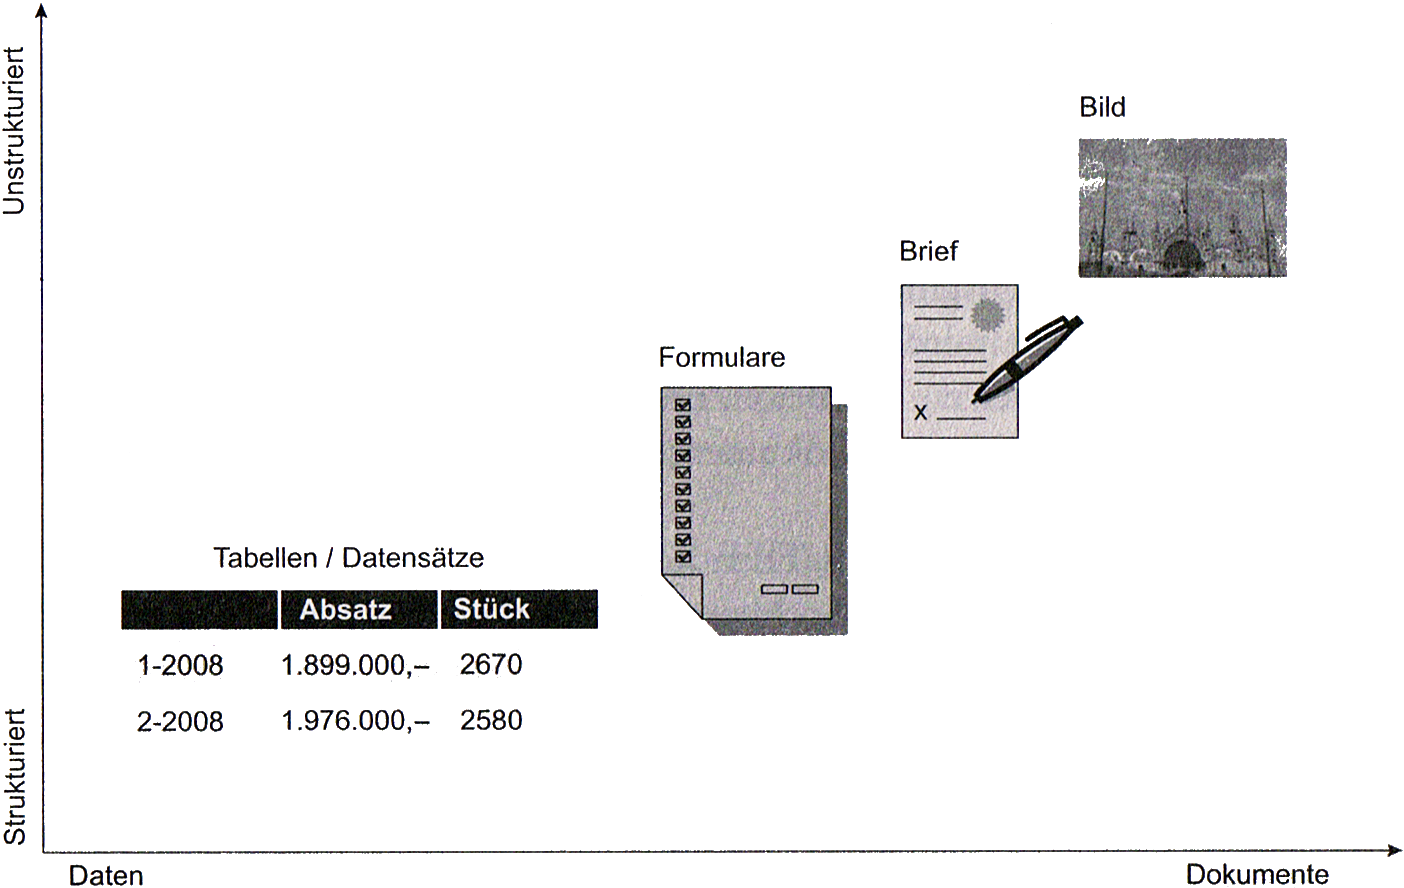
\includegraphics[width=0.85\textwidth]{bilder/cci4.png}}
		\caption[Anteil an strukturierten Informationen]{Anteil an strukturierten Informationen\protect\footnote}
		\label{ncici}
\end{figure}
\footnotetext{Quelle: \cite{DMS08} S. 33}

Unter \textbf{Dokumenten-Management} werden primär die Verwaltungsfunktionen Erfassung, Bearbeitung, Verwaltung und Speicherung von Dokumenten verstanden. \cite{DMS08} S. 344.\newpage

Darunter fallen laut \cite{DMS08} S. 3 folgende Punkte:

\begin{itemize}
\item Kennzeichnung und Beschreibung von Dokumenten (auch Metadaten des Dokuments genannt) 
\item Fortschreibung, Versionierung und Historienverwaltung von Dokumenten
\item Ablage und Archivierung von Dokumenten
\item Verteilung und Umlauf von Dokumenten
\item Suche nach Dokumenten bzw. Dokumenteninhalten
\item Schutz der Dokumente vor Verfälschung, Missbrauch und Vernichtung
\item Langfristiger Zugriff auf die Dokumente und Lesbarkeit der Dokumente
\item Lebenslauf und Vernichtung von Dokumenten
\item Regelung von Verantwortlichkeiten für Inhalt und Verwaltung von Dokumenten
\end{itemize}
%\newpage
Der Begriff \textbf{"`Dokumenten-Management-System"'} muss auch in zwei verschiedene Sichtweisen differenziert werden:
\begin{quote}"`Bei \textbf{Dokumenten-Management-Systemen im engeren Sinne} geht es um die Logik der Verwaltung von Dokumenten, deren Status, Struktur, Lebenszyklus und Inhalt. Dokumente werden beschrieben, klassifiziert und in einer bestimmten logischen Struktur eingeordnet, damit sie einfach wieder gefunden werden können. Dokumente entstehen, werden verändert und (irgendwann) vernichtet.

Den \textbf{Dokumenten-Management-Systemen im weiteren Sinne} ordnet man auch noch weitere Funktionalitäten zu, wie z. B. Schrifterkennung, automatische Indizierung, [...], Publizierung. Hier lassen sich die Grenzen nicht mehr genau bestimmten!"' \begin{flushright}\cite{DMS08} S. 5\end{flushright}\end{quote}

Die Grundstruktur eines Dokumenten-Management-Systemes kann man dadurch grob in folgender Abbildung zusammenfassen:
\begin{figure}[ht]
	\centering
	   \fbox{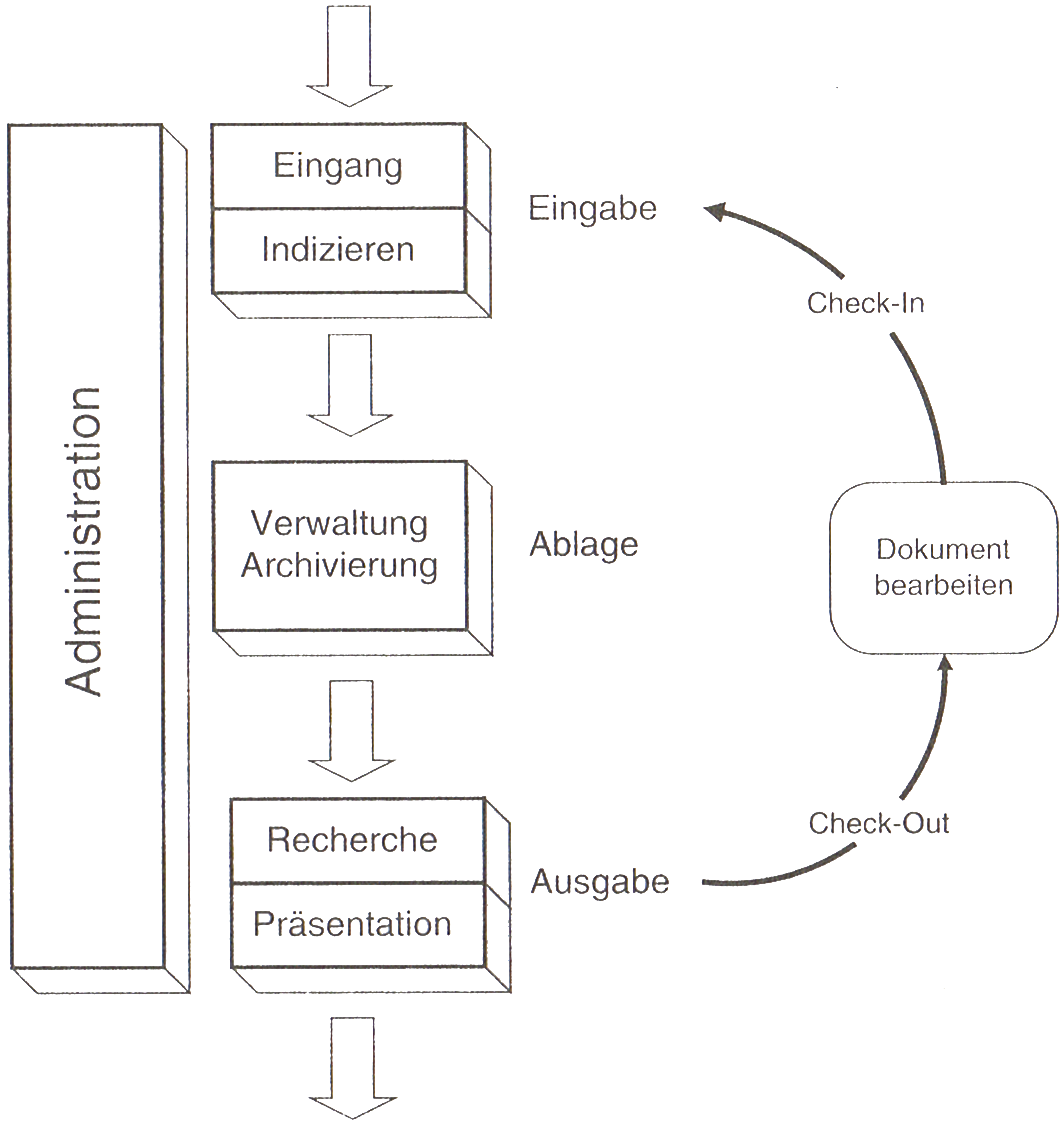
\includegraphics[width=0.57\textwidth]{bilder/3aufgaben.png}}
		\caption[Aufgabenbereiche eines Dokumenten-Management-Systems]{Aufgabenbereiche eines Dokumenten-Management-Systems\protect\footnote}
		\label{lifecircle}
\end{figure} 
\footnotetext{Quelle: \cite{DMS08} S. 38}

Dabei wird ein \gls{DMS}-System in drei verschiedene Teilbereiche aufgegliedert:

\subsubsection{Eingabe}
Unabhängig des Ursprungs oder der Art des Dokumentes besitzt der Funktionsbereich Eingabe die Aufgabe diese Dokumente dem Dokumenten-Management-System zuzuführen.
%(Darunter fallen auch Post, Email, Andere Anwendungen, fax usw. - Hier Hinweis auf WSDL)

Laut \cite{DMS08} S. 40fff fallen in diesen Bereich zwei Funktionen:

\paragraph{Dokumenteneingang}
Hier wird die Zuspielung der Dokumente in das \gls{DMS}-System durch verschiedene Methoden realisiert.
Als mögliche Eingabe von Dokumenten kann sowohl das Einscannen von Textdokumente oder Bilder als auch der elektronische Eingang von Dokumenten durch E-Mail oder externen Anwendungen fungieren.

Auch hier gilt zu unterscheiden, dass durch den Einscannvorgang erstellte Dokumente als \gls{NCI}-Dokument abgelegt werden und bereits digitalisierte Dokumente sich zur Umwandlung zu \gls{CI}-Dokumenten anbieten.
Sobald der Inhalt von eingescannten Dokumenten zur weiteren Verarbeitung ausgelesen bzw. ausgewertet werden soll, müssen die Dokumente in ein \gls{CI}-Format transformiert werden.
Dies wird häufig durch eine \gls{OCR}-Software realisiert, die beispielsweise das Bild eines eingescannten Briefes in Text umwandelt.

Bereits im \gls{CI}-Format vorliegende Dokumente müssen nicht transformiert werden, jedoch werden die Dokumente oft in anderen Formaten zusätzlich abgespeichert.
Ein Beispiel ist die Umwandlung eines Microsoft Word-Dokumentes in ein \gls{PDF}-Dokument oder von unterschiedlichen Bildformaten in ein einheitliches Format.

\paragraph{Indizierung}
Bei der Indizierung werden Dokumente zur eindeutigen Identifikation mit Attributen versehen.
Diese Attribute werden teilweise automatisch durch das \gls{DMS}-System anhand einer hoch zählenden Identifikationsnummer oder manuell durch den Benutzer beim Einstellen des Dokumentes hinzugefügt.
Solche Attribute werden auch als Metadaten des Dokumentes bezeichnet und meist als zusätzliche Suchkriterien angeboten.

Dabei werden in \cite{DMS08} S. 44 zwei verschiedene Methoden zur automatischen Klassifizierung genannt.
Beim wissensbasiertem Ansatz wird mittels umfangreichem Wissen über das Umfeld der Dokumente und dadurch abgeleitete Regeln dem System ermöglicht diese Dokumente automatisch einzuordnen und zu indizieren.
Eine weitere Möglichkeit eröffnet sich durch das Verwenden von neuronalen Netzen.
Hierbei wird durch die Vorarbeit eines Menschen Beispiele geschaffen anhand welcher sich das System selbstständig Auswahlkriterien erzeugt.
Je mehr korrekte Beispiele vorgegeben werden, desto besser und zuverlässiger arbeitet die automatische Klassifizierung.

\subsubsection{Verwaltung und Archivierung}
Bei der \textbf{Verwaltung} werden die Probleme beim \textit{Check-in} (Einspielen des Dokumentes), Bearbeitung und \textit{Check-out} (Signalisieren der Weiterbearbeitung) behandelt, siehe auch Abbildung \ref{lifecircle}.
Wie auch bei einer Datenbank müssen Dokumente, die gerade bearbeitet werden, für andere Benutzer für Änderungen gesperrt werden, damit keine Inkonsistenzen auftreten können.
Nach einer Bearbeitung und dem Check-in des abgeänderten Dokumentes muss die Versionsverwaltung des \gls{DMS}-Systems beide Versionen beibehalten und (dabei) die ursprüngliche Version als veraltet und die neue Version als solche kennzeichnen.
Zusätzlich muss die Wiederherstellung einer älteren Revision als aktuelles Dokument unterstützt werden.


Die \textbf{Archivierung} befasst sich mit der Sicherung und Wiederherstellung von Dokumenten und deren Metadaten.
Im Zusammenhang mit DMS-Systemen springt man auch von einer revisionssicheren Archivierung.
Dabei müssen laut \cite{DMS08} S. 288 unter anderem bestimmte Punkte eingehalten werden:

\begin{itemize}
\item Jedes Dokument muss unveränderbar archiviert werden.
\item Es darf kein Dokument auf dem Weg ins Archiv oder im Archiv selbst verloren gehen.
\item Kein Dokument darf während seiner vorgesehenen Lebenszeit zerstört werden können.
\item Jedes Dokument muss in genau der gleichen Form, wie es erfasst wurde, wieder angezeigt und gedruckt werden können.
\end{itemize}

\subsubsection{Ausgabe}
Wie die Eingabe besteht die Ausgabe aus zwei Funktionen:

\paragraph{Recherche}
Die Recherche ist die Suche nach einem Dokument entweder durch eine strukturierte Suche anhand von zuvor eingetragenen Attributen (Autor, Erstellungsdatum, Speichergröße usw.) oder durch eine Volltextsuche.

Die \textbf{strukturierte Suche} ist nur bei einer qualitativ hochwertigen Indizierung effizient, bietet dafür auch mit guter zeitlichen Performanz die besten Ergebnisse, sofern die Indizierung entsprechend eingehalten wurde.

Die \textbf{Volltextsuche} besteht aus einer ordinären Suche durch den Inhalt der Dokumente nach den eingegebenen Suchbegriffen.
Daher ist die Qualität der Suchergebnisse unabhängig von der Qualität der Indizierung.
Jedoch können nur \gls{CI}-Dokumente, deren Informationen auch durch den Computer auslesbar und interpretierbar sind, durchsucht werden.
\gls{NCI}-Dokumente wie Bilder oder Videos können ohne Metadaten durch die Volltextsuche nicht gefunden werden.

\paragraph{Reproduktion}
In diesem Teilbereich können die gespeicherten Dokumente wieder vom Benutzer abgerufen werden.
Dies ist durch eine einfach Anzeige im Webbrowser, eine Weiterleitung per E-Mail oder eine Sendung als Druckauftrag möglich.



\subsection{Content-Management-Systeme}
Bei einem Content-Management-System (\gls{CMS})  steht nicht mehr das eigentliche Dokument im Vordergrund, sondern vielmehr der enthaltene Informationsgehalt des Dokuments. \newpage
Der Unterschied zwischen einem \gls{DMS} und einem \gls{CMS} besteht laut \cite{DMS08} S. 114 im folgenden:

%Abgrenzend zum Dokumenten-Management handelt es sich beim Content-Management nicht vordergründig um die Verwaltung von Dokumenten, sondern um die Verwaltung von Informationseinheiten, die miteinander verknüpft sein können. [...] Je nach Ausprägung kann nun ein konkretes System als Dokumenten-Management-System mit Content-Management-Funktionen definiert werden und umgekehrt. [...]

%Der Ansatz des Content-Management unterscheidet sich vom "`klassischen"' Dokumenten-Mangement vor allem in Bezug auf die betrachteten Objekte: 
\begin{quote}"`Ein \gls{DMS} hat als kleinstes Objekt der Betrachtung eines einzelnen Dokument. [...] Content-Management ist auf logische Informationseinheiten ausgerichtet. Es ist z.B. das Ziel des Content-Managements, Inhalte, die auf mehrere Quellen verteilt sind, neue zusammenzustellen und daraus z.B. ein neues Dokument zu generieren."'
\begin{flushright}\cite{DMS08} S. 114f\end{flushright}\end{quote}

Die folgende Abbildung soll den charakteristischen Unterschied zwischen \gls{CMS}-Systemen und \gls{DMS}-Systemen verdeutlichen.


\begin{figure}[ht]
	\centering
	   \fbox{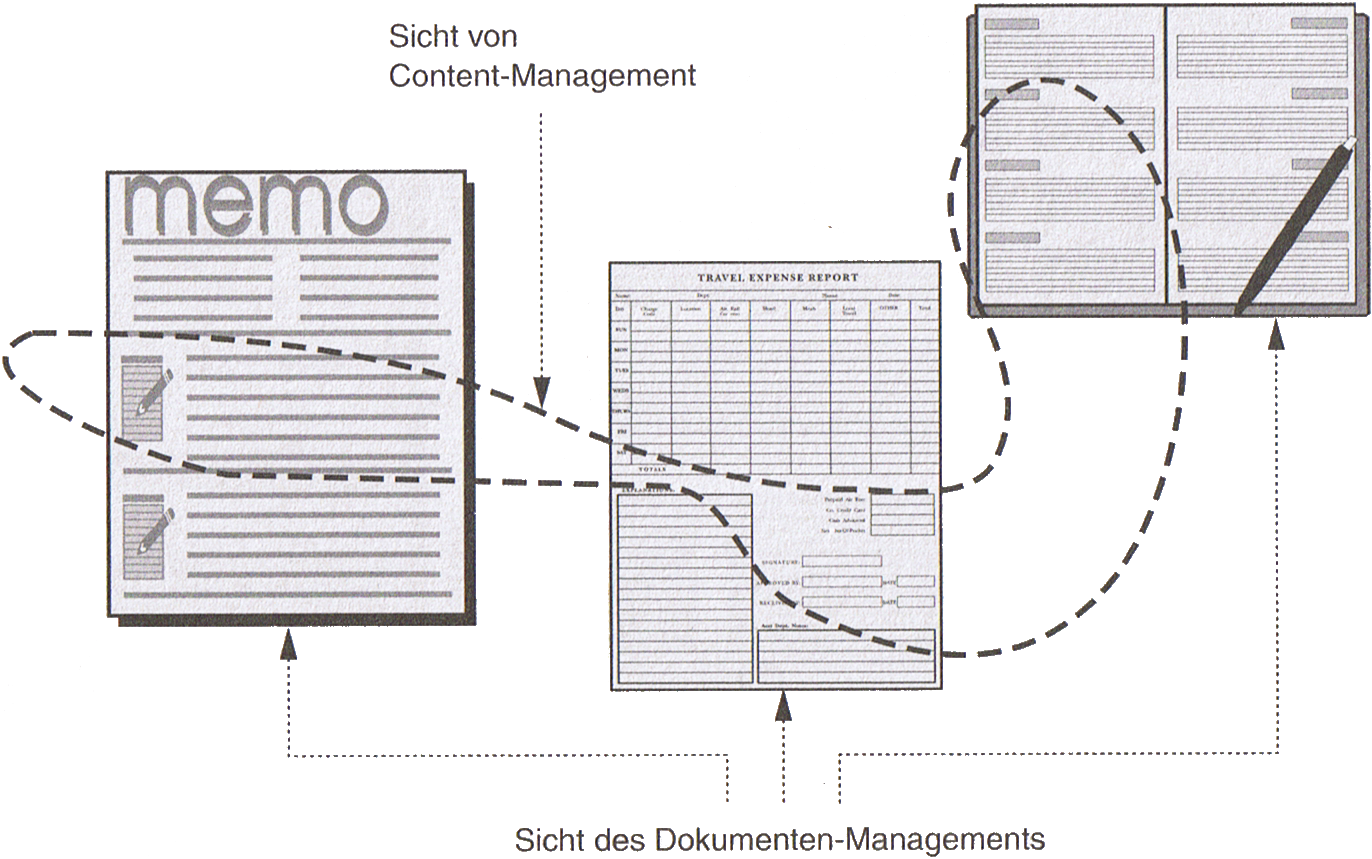
\includegraphics[scale=0.9]{bilder/cmsdms3.png}}
		\caption[Sichtweise CMS gegenüber DMS]{Sichtweise CMS gegenüber DMS\protect\footnote}
		\label{dmsvscms}
\end{figure} 
\footnotetext{Quelle: \cite{DMS08} S. 115}


Wie zuvor beschrieben ist die Sichtweise eines \gls{DMS} nur auf die einzelnen Dokumente beschränkt, während ein \gls{CMS} einzelne Elemente aus den Dokumenten extrahieren und ggf. zu einem neuen Dokument verschmelzen kann. Die Sichtweise des \gls{CMS} wird durch das gestrichelte Polygon dargestellt, welches hier dokumentenübergreifend abgebildet ist.

Das Ziel eines \gls{CMS}-Systems ist laut Oracle folgendermaßen definiert:

\begin{quote}"`The key to a successful content management implementation is unlocking the value of content by making it as easy as possible for it to be consumed. This means that any piece of content must be available to any consumer, no matter what their method of access."'
\begin{flushright}\cite{UCM07} S. 12\end{flushright}\end{quote}

Ein \gls{CMS} soll jede Darstellungsart von Informationen aufnehmen und jedes Element dieser Information den Benutzern zugänglich machen, unabhängig von der Art des Zugriffs.
Dieses Konzept soll in Abbildung \ref{ucm-a2a} verdeutlicht werden.

\begin{figure}[ht]
	\centering
	   \fbox{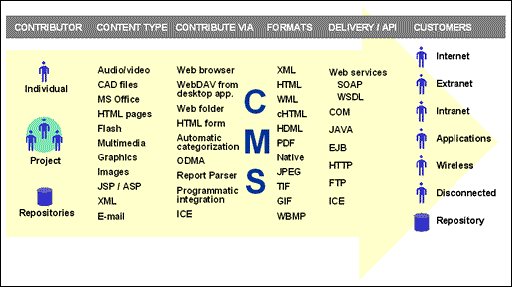
\includegraphics[width=0.8\textwidth]{bilder/ucm.png}}
		\caption["`any-to-any"' Content-Management Konzept]{"`any-to-any"' Content-Management Konzept\protect\footnote}
		\label{ucm-a2a}
\end{figure}
\footnotetext{Quelle: \cite{UCM07} S. 12}

Das \gls{CMS} steht hier in der Mitte der Abbildung als Medium zwischen den verschiedenen Inhalten, eingestellt von den \textit{Contributors} (links), und den Anwendern, die auf transformierte Versionen der Inhalte durch unterschiedliche Arten zugreifen (rechts).


\subsection{Enterprise-Content-Management-Systeme}
Der Begriff Enterprise-Content-Management (\gls{ECM}) wird auch häufig in Verbindung mit \gls{CMS}-Systemen und \gls{DMS}-Systemen genannt.
Laut der "`Association for Information and Image Management"' (\gls{AIIM}\footnote{Die AIIM ist eine Gesellschaft von internationalen Herstellern und Anwendern von Informations- und Dokumenten-Mangement-Systemen}) umfasst dieser Begriff die Verwaltungsfunktionen von Unternehmensinformationen in unterschiedlichen Dokumentformaten.\footnote{Quelle: \url{http://www.aiim.org/What-is-ECM-Enterprise-Content-Management.aspx}}
Diese Funktionen werden laut \cite{DMS08} S. 116 durch verschiedene "`Systeme wie Dokumenten-Management, Groupware, Workflow, Input- und Output-Management, (Web-)Content-management, Archivierung, Records-Management und andere"' bereitsgestellt.


%\subsection{Universal-Content-Management-Systeme}
%Im Gegensatz zu anderen \gls{CMS}-Systemen, wie Typo3 oder Joomla, bezeichnet Oracle seine Softwarelösung in diesem Bereich als Universal-Content-Management (\gls{UCM}).
%Jedoch unterscheidet es sich in der technisches Umsetzung nicht von anderen \gls{CMS}-Systemen.
%Es wir vermutet, dass sich Oracle durch diese Bezeichnung von den anderen \gls{CMS}-Systemen abheben / absetzten wollte, also nur aufgrund von Marketing-Vorteilen ihr Produkt so nannte.





















\subsection{Service-Orientierte Architektur}
Ein Versuch einer Definition erhält man aus \cite{SOA07} S. 27:
\begin{quote}"`[...] a service oriented architecure is an architecture for building buisness applications as a set of loosley coupled black-box components orchestrated to deliver a well-defined level of service by linking together business processes"' \begin{flushright}\cite{SOA07} S. 27\end{flushright}\end{quote}
Service-Oriented Architecture (\gls{SOA}) ist ein Ansatz im Bereich der Informationstechnik um Anwendungen oder einzelne Dienste aus verschiedenen Geschäftsprozessen zu bilden.



Zur Verdeutlichung kann ein beispielhafter und vereinfachter Aufbau eines Online-Shops genommen werden.

\begin{figure}[ht]
	\centering
	   \fbox{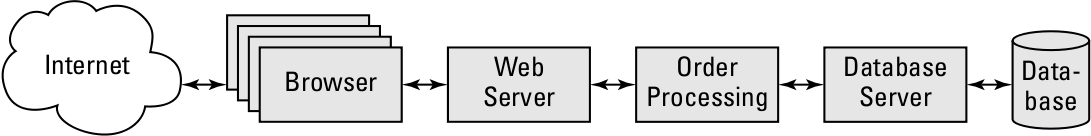
\includegraphics[width=0.85\textwidth]{bilder/soa1.png}}
		\caption[Einfach Software Architektur]{Einfach Software Architektur\protect\footnote}
		\label{soa1}
\end{figure}
\footnotetext{Quelle: \cite{SOA07} S. 18}
Durch den gewöhnlichen Browser können Benutzer auf die Webseite des Webservers zugreifen um dort auf die eigentliche Anwendung des Webshops \textit{Order Processing} zuzugreifen.
Dabei werden durch einen Datenbankserver die Informationen in einer Datenbank gespeichert oder von dort der Webshop-Anwendung zugänglich gemacht.
Welche Funktion die Anwendung \textit{Order Processing} ausführt hängt von den Aufforderungen des Benutzers durch den Browser ab.

Dieser Struktur wird nun ein Service-Orientierte Komponente \textit{Credit Checking} hinzugefügt, siehe Abbildung \ref{soa2}.

\begin{figure}[ht]
	\centering
	   \fbox{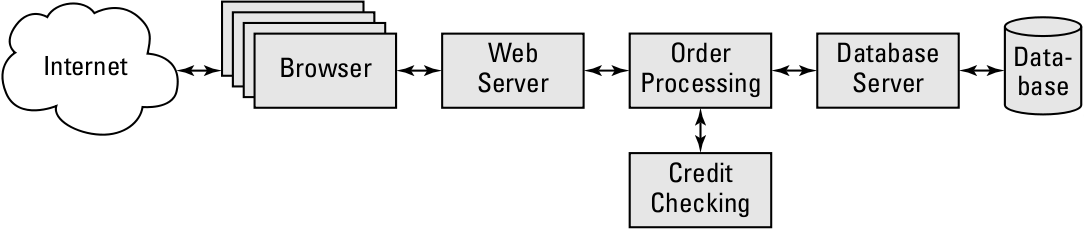
\includegraphics[width=0.85\textwidth]{bilder/soa2.png}}
		\caption[Erweiterte Software Architektur mit Service-Orientierte Komponente]{Erweiterte Software Architektur mit Service-Orientierte Komponente\protect\footnote}
		\label{soa2}
\end{figure}
\footnotetext{Quelle: \cite{SOA07} S. 20}

Dabei hat die eigentliche Anwendung des Webshops keine Kenntniss wie die Komponente \textit{Credit Checking} intern abläuft, sondern übergibt nur die essentiellen Informationen, in diesem Fall die Kreditkartendaten, an die Komponente.
Es ist unrelevant, ob diese Komponenten eine externe Datenbank oder Webseite nach der Kreditwürdigkeit des Benutzers befragen, solange die Komponente auswertbare Informationen (zahlungsfähig ja/nein) an die Webshop Anwendung liefert.
Für die Anwendung \textit{Order Processing} ist die Komponente \textit{Credit Checking} eine sogennante \textbf{black box}.

Die komplexen Berechnungen und Algorithmen zur Bestimmung der Kreditwürdigkeit des Benutzers werden komplett verdeckt, so dass nur die Kreditkarteninformationen der Komponente zu übergeben sind.

Die Komponente \textit{Credit Checking} steht der Webshop Anwendung als \textbf{abstrahierter Dienst bzw. Service} zur Verfügung.

%\subsection{[cronjobs]}

%\subsection{[Farbraum]}
%\subsection{[ds - ADS Benutzer]}
%\subsection{[Metadaten allg]}
%\subsection{[alse+-true+-]}
%\subsection{[evtl Oracle DB]}







 \newpage
\section{Umsetzung}
In diesem Kapitel wird die Vorgehensweise der zuvor beschriebenen Problemstellungen erörtert.

\subsection{Aufbau der Testumgebung}




\subsubsection{Aufsetzen eines Nagios-Test-Systems}
Da die einzelnen Überwachungselemente in der Überwachungssoftware Nagios nach und nach eingetragen (/ definiert / assoziiert / verbunden) werden müssen, ist ein häufiges Neustarten der Nagios Anwendung notwendig, damit die neuen Konfigurationsdateien übernommen werden.

Damit dies nicht auf dem produktiven Nagios-Server durchgeführt werden muss, wird ein Nagios-Testserver für diesen Zwecks eingesetzt.

\subsubsection{Bilddatenbank als VM}
Für die Simulation der verschiedenen Fehlerzuständen der einzelnen Überwachungselemente wird eine virtuelle Maschine mit einer \gls{OracleUCM} Prototypinstallation, die extra als Entwicklungsplattform erstellt wurde, verwendet.


\subsection{Basisüberwachung - Konfigurationsdateien}
\begin{itemize}
\item Wie/wo werden Hosts eingetragen -> hostgroups
\item Service Definitionen -> mit Host verbinden
\item Wer wird wann wegen was wie benachrichtigt -> contacts
\end{itemize}



\subsection{Einrichten des Windows Agenten}
\begin{itemize}
\item Port ändern -> RPC
\item Verschlüsselung durch PW und/oder Algo
\item Hinzufügen der Plugins
\item Bsp Aufruf aktiver Check
\end{itemize}

.Net 2.0 Framework essentiell
NC\_Net installieren
nagios server ip zur sicherheit angeben
port ändern
pw hinzufügen
-> dienst starten

test vom nagios host:

\begin{lstlisting}[captionpos=b, caption=Aufruf eines aktiven Checks, label=activecheckexample, breaklines = true]
root@iwrpaul:/usr/local/nagios/libexec# ./check_nc_net -H secret.kit.edu -p 123456 -s secret -v RUNSCRIPT -l check_uname.exe
Operating System OK - Microsoft(R) Windows(R) Server 2003 Standard Edition Service Pack 2
\end{lstlisting}

Das auf dem Nagios Server liegende Script \pictext{check\_nc\_net} stellt eine Verbindung zum angegebenen Server her und führt die mit dem Parameter \pictext{l} angegebene Datei aus. Dafür muss sich diese Datei in dem Script Verzeichnis des NC\_Net befinden.


Danach command definition hinzufügen, weil PW und Port verändert wurde:
\begin{lstlisting}[captionpos=b, caption=Nagios-Befehls Definition für den Host, label=activecheckexample, breaklines = true, language=sh]
# 'check_nt_bdb' command definition
#	_NSCLIENT_PORT	13599
#	_NSCLIENT_PW	KAnqloaQk
#
define command{
    command_name    check_nc_net_bdb
	command_line 	/usr/lib/nagios/plugins/check_nc_net -H $HOSTNAME$ -p 13599 -s KAnqloaQk -v $ARG1$
        }
\end{lstlisting}

Danach
\begin{itemize}
\item Logfiles check.exe 
\item batchloader.exe script
\end{itemize}


\subsection{Überprüfen der Prozesse und Services}
\begin{itemize}
\item Prozesse
\item Services
\item Bsp Aufruf
\end{itemize}

\subsection{Umsetzung der Funktionlitätstest}
\begin{itemize}
\item batchloader + .blo Dateien
\item einloggen mit lokalem und ads benutzer
\end{itemize}

\gls{SOA} steht für Service-Oriented Architecture und benutzt das Simple Object Access Protocol (\gls{SOAP}), welches ein \gls{XML}-basierendes Protokoll zur Ausführung von Programmen / Befehle auf entfernten Rechnern ist.

\subsection{Auswertung der Logs + Stopwörterdefinition}
\begin{itemize}
\item check\_logfiles
\item check\_logfiles cfg file inkl. Rotation
\end{itemize}

\subsection{Benutzersimulation}
\begin{itemize}
\item \url{http://www.w3schools.com/soap/default.asp} Web Services und SOAP
\item \url{http://www.w3schools.com/wsdl/wsdl_summary.asp} WSDL
\item max attempts bei Search erhöhen, da Auslastung der InboundRef -> möglichst keine/geringe False Positives -> auf Ausblick verweisen, Rahmenbedingungen müssen im Feld in der Praxis erst noch gefunden werden
\end{itemize}

\begin{figure}[ht]
	\centering
	   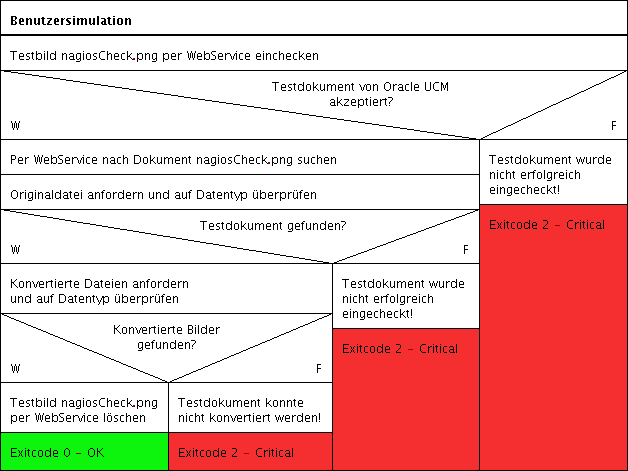
\includegraphics[width=0.9\textwidth]{bilder/Benutzersimulation.png}
		\caption{Ablauf der Benutzersimulation}
		\label{user-sim}
\end{figure}
 \newpage
%\input{/16/docs/_praxis3/tex/ziele.tex} \newpage
%\input{/16/docs/_praxis3/tex/programmaufbau.tex} \newpage
%\input{tex/anpassungen.tex} \newpage
%\section{Zusammenfassung und Ausblick}

\begin{itemize}
\item Geeignete Stopwörter für Logdateien müssen noch gefunden / eruiert werden
\item Passende Schwellwertdefinitionen können erst nach einer gewissen Laufzeit festegelegt werden
\item Export der entwickelten Überwachung auf den produktiven Haupt-Nagios Server
\end{itemize} \newpage
%\section{Einleitung}

Einleitung halt.
Kurz was ist Nagios, warum überhaupt überwachen?
Was soll überwacht werden -> Stellent/UCM kurz was ist das? Warum gerade das überwachen -> Aktive Benutzung durch User - kritisch \newpage
%\section{Einleitung}

Einleitung halt.
Kurz was ist Nagios, warum überhaupt überwachen?
Was soll überwacht werden -> Stellent/UCM kurz was ist das? Warum gerade das überwachen -> Aktive Benutzung durch User - kritisch 

%\newpage
\section{Anhang}
\subsection{Abbildungsverzeichnis}
\listoffigures

\newpage

\renewcommand{\lstlistlistingname}{}
\subsection{Codelistingverzeichnis}
\lstlistoflistings
\newpage


\renewcommand{\refname}{} 
\subsection{Literaturverzeichnis}
\begin{thebibliography}{xxxxxxxx}
	 \bibitem[DMS08]{DMS08}Götzer, Klaus; Schmale, Ralf; u.a. (2008) "`Dokumenten-Management - Informationen im Internehmen effizient nutzen"' 4. Auflage,\\
	 dpunkt.verlag GmbH Heidelberg,  
	 ISBN13: 978-3-89864-529-4,\\
	 Stand: ????, Einsichtnahme: 05.06.2009

	 \bibitem[Barth08]{Barth08}Wolfgang Barth (2008) "`Nagios - System- und Netzwerk-Monitoring"' 2. Auflage, \\
	 ISBN13: 978-3-937514-46-8, \\
	 Stand: ????, Einsichtnahme: 14.05.2009
	 
	 \bibitem[Huff06]{Huff06}Brian Huff (2006) "`The Definitive Guide to Stellent Content Server Development"', \newline ISBN13: 978-1-59059-684-5, \newline Stand: ????, Einsichtnahme: 15.05.2009
	 
	 	 \bibitem[UCMlog09]{UCMlog09} Unbekannter Author "`vramanat"' (2009) "`Universal Content Management 10gR3 - Content Server Log File Information"', \\ Quelle: \url{http://www.oracle.com/technology/products/content-management/cdbs/loginfo.pdf} \newline Stand: 20.01.2009, Einsichtnahme: 05.06.2009
\end{thebibliography}
\newpage
\subsection{Glossar}
\renewcommand{\glossaryname}{}
\makeglossaries
\printglossaries

\end{document}



